\documentclass[letterpaper,10pt]{article}

%\setlength{\parindent}{0in}
%\usepackage{fullpage} 
\usepackage{amsmath}
\usepackage{enumerate}
\usepackage{graphicx}
\oddsidemargin 0.0in
\textwidth 6.5in

%opening
\title{Homework for Module 9}
\author{Steve Mazza}

\begin{document}
\maketitle

\begin{description}
\item[11.1.3]\ 
\begin{table}[htdp]
\caption{Analysis of variance table}
\begin{center}
\begin{tabular}{l|rrrrr}
\textbf{Source} & \textbf{Degrees of Freedom} & \textbf{Sum of Squares} & \textbf{Mean Squares} & \textbf{$F$-statistic} & \textbf{$p$-value} \\
\hline \textbf{Treatments} & 7 & 126.95 & 18.14 & 5.01 & 0.002 \\
\textbf{Error} & 22 & 79.64 & 3.62 & & \\
\hline \textbf{Total} & 29 & 206.59 & & & 
\end{tabular}
\end{center}
\label{default}
\end{table}

\item[12.1.1]\ 
\begin{enumerate}[a)]
\item 21.2
\item 5.1
\item 0.59
\item 0.4
\item 0.35
\end{enumerate}

\item[12.2.4]\ 
\begin{enumerate}[a)]
\item \ 
\begin{center}
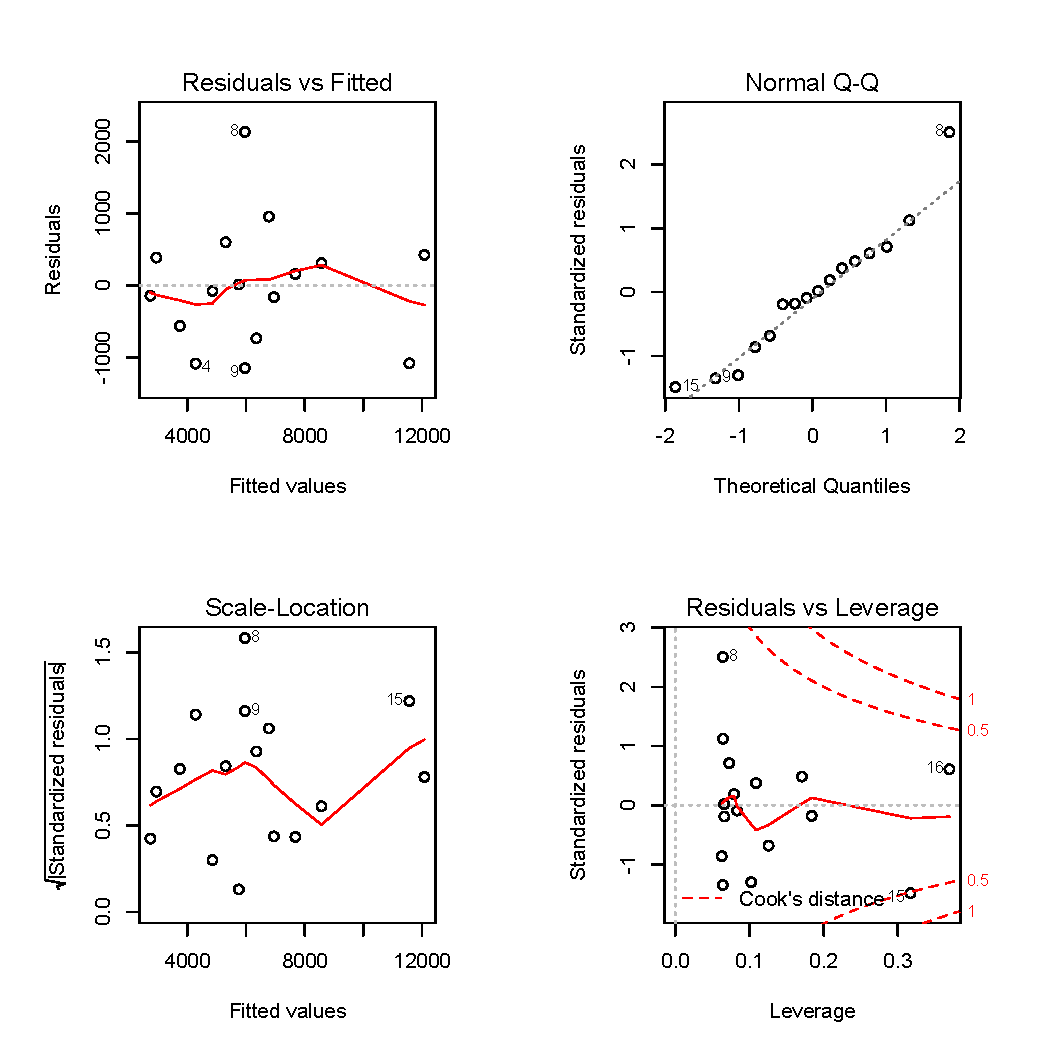
\includegraphics[scale=0.75]{module9a.pdf}
\end{center}
\item
\item \$7756.321K
\item \$879.9K
\item \$17789.711K
\end{enumerate}

\item[12.3.3]\ 
\begin{enumerate}[a)]
\item $8.532\times10^{-2}$
\item $(0.82, 1.19)$
\item $t$-value = 11.76 and the $p$-value = $1.212\times10^{-8}$
\end{enumerate}

\item[12.4.4]\ 
fit: 7254.651, lower: 6754.55, upper: 7754.752

\item[12.5.3]\ 
(5302, 9207)

\item[12.6.5]\ 
\begin{table}[htdp]
\caption{Analysis of variance table}
\begin{center}
\begin{tabular}{l|rrrrr}
\textbf{Source} & \textbf{Degrees of Freedom} & \textbf{Sum of Squares} & \textbf{Mean Squares} & \textbf{$F$-statistic} & \textbf{$p$-value} \\
\hline \textbf{Regression} & 1 & $10.71\times10^{7}$ & $10.71\times10^{7}$ & 138.29 & 0.0 \\
\textbf{Error} & 14 & $1\times10^{7}$ & 774,211 & & \\
\hline \textbf{Total} & 15 & $11.79\times10^{7}$ & & & 
\end{tabular}
\end{center}
\label{default}
\end{table}

\item[12.7.1]\ 
No.

\item[12.11.14]\ 
Yes.

\end {description}
\end{document}